\section*{Bài 3}

Chứng minh đa thức $f \big( x \big) = x^3 - x + 1$ có 3 nghiệm phân biệt. Tính giá trị: $S = {x_1}^8 + {x_2}^8 + {x_3}^8$ với $x_1, x_2, x_3$ là 3 nghiệm của $f \big( x \big)$.

\begin{center}
    \textbf{\underline{Bài làm:}}
\end{center}

Ta sử dụng \textbf{Maple} để tìm nghiệm của phương trình trên.

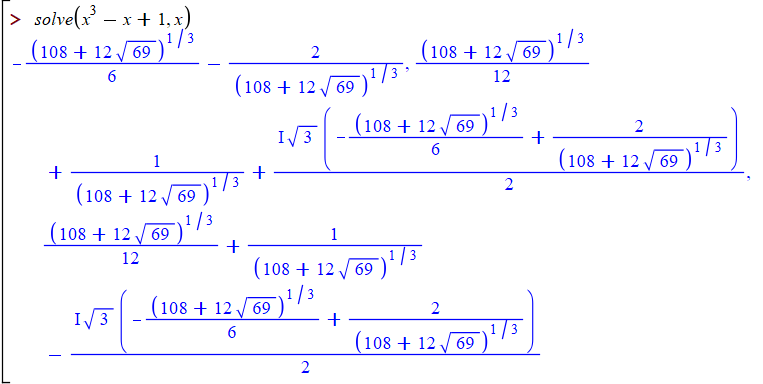
\includegraphics[width=1.0\textwidth]{bai3.png}

Như vậy, ta thấy phương trình trên có 3 nghiệm phân biệt.

Theo định lí Vi-et với phương trình bậc 3, ta có:

$\begin{cases}
    \displaystyle
    x_1 + x_2 + x_3 = - \frac{b}{a} = - \frac{0}{1} = 0\\
    \displaystyle
    x_1 x_2 + x_2 x_3 + x_3 x_1 = \frac{c}{a} = \frac{-1}{1} = -1\\
    \displaystyle
    x_1 x_2 x_3 = - \frac{d}{a} = - \frac{1}{1} = -1
\end{cases}$

Đặt $t_1 = {x_1}^4, t_2 = {x_2}^4, t_3 = {x_3}^4$, ta được:

$S = {t_1}^2 + {t_2}^2 + {t_3}^2\\ = (t_1 + t_2 + t_3)^2 - 2(t_1 t_2 + t_2 t_3 + t_3 t_1)\\ = \left( {x_1}^4 + {x_2}^4 + {x_3}^4 \right)^2 - 2 \big[ (x_1 x_2)^4 + (x_2 x_3)^4 + (x_3 x_1)^4 \big]$

Mà:

$(x_1 x_2)^2 + (x_2 x_3)^2 + (x_3 x_1)^2\\
= (x_1 x_2 + x_2 x_3 + x_3 x_1)^2 - 2 x_1 x_2 x_3 (x_1 + x_2 + x_3) = (-1)^2 - 2 \cftdot (-1) \cftdot 0 = 1$

$(x_1 x_2)^4 + (x_2 x_3)^4 + (x_3 x_1)^4\\ = \big[ (x_1 x_2)^2 + (x_2 x_3)^2 + (x_3 x_1)^2 \big] ^2 - 2 (x_1 x_2 x_3)^2 ({x_1}^2 + {x_2}^2 + {x_3}^2)\\ = \big[ (x_1 x_2)^2 + (x_2 x_3)^2 + (x_3 x_1)^2 \big] ^2 - 2 (x_1 x_2 x_3)^2 \big[ (x_1 + x_2 + x_3)^2 - 2(x_1 x_2 + x_2 x_3 + x_3 x_1) \big] = 1^2 - 2 \cftdot (-1)^2 \cftdot \big[ 0^2 - 2 \cftdot (-1) \big] = -3$

${x_1}^4 + {x_2}^4 + {x_3}^4\\ = (x_1 + x_2 + x_3)^4 + 4(x_1 x_2 + x_2 x_3 + x_3 x_1)^2 -4(x_1 x_2 + x_2 x_3 + x_3 x_1)(x_1 + x_2 + x_3)^2 - 2 \big[ (x_1 x_2)^2 + (x_2 x_3)^2 + (x_3 x_1)^2 \big]\\ = 0^4 + 4 \cftdot (-1)^2 - 4 \cftdot (-1) \cftdot 0^2 - 2 \cftdot 1 = 2$

Vậy $S = 2^2 - 2 \cftdot (-3) = 10$.
	
\addcontentsline{toc}{section}{Bài 3}

\clearpage